% \iffalse
\let\negmedspace\undefined
\let\negthickspace\undefined
\documentclass[journal,12pt,twocolumn]{IEEEtran}
\usepackage{cite}
\usepackage{amsmath,amssymb,amsfonts,amsthm}
\usepackage{algorithmic}
\usepackage{graphicx}
\usepackage{textcomp}
\usepackage{xcolor}
\usepackage{txfonts}
\usepackage{listings}
\usepackage{enumitem}
\usepackage{mathtools}
\usepackage{gensymb}
\usepackage{comment}
\usepackage[breaklinks=true]{hyperref}
\usepackage{tkz-euclide} 
\usepackage{listings}
\usepackage{gvv}                                        
\def\inputGnumericTable{}                                 
\usepackage[latin1]{inputenc}                                
\usepackage{color}                                            
\usepackage{array}                                            
\usepackage{longtable}                                       
\usepackage{calc}                                             
\usepackage{multirow}                                         
\usepackage{hhline}                                           
\usepackage{ifthen}                                           
\usepackage{lscape}
\newtheorem{theorem}{Theorem}[section]
\newtheorem{problem}{Problem}
\newtheorem{proposition}{Proposition}[section]
\newtheorem{lemma}{Lemma}[section]
\newtheorem{corollary}[theorem]{Corollary}
\newtheorem{example}{Example}[section]
\newtheorem{definition}[problem]{Definition}
\newcommand{\BEQA}{\begin{eqnarray}}
\newcommand{\EEQA}{\end{eqnarray}}
\newcommand{\define}{\stackrel{\triangle}{=}}
\theoremstyle{remark}

\newtheorem{rem}{Remark}
\begin{document}
\parindent 0px
\bibliographystyle{IEEEtran}
\title{Assignment 10.5.3\_18Q}
\author{EE23BTECH11028 - Kamale Goutham$^{}$% <-this % stops a space
}
\maketitle
\newpage
\bigskip
\textbf{Question}
A spiral is made up of successive semicircles,with centres alternately at A and B,starting with centre at A,of radii $0.5cm,1.0cm,1.5cm,2.0cm$,... as shown in Fig.$5.4$.what is the total length of such a spiral made up of thirteen consecutive semicircles?(Take $\pi=\frac{22}{7}$)\\
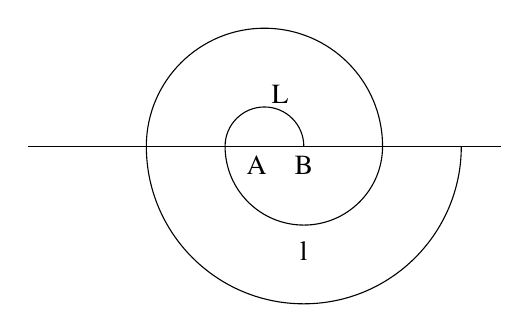
\begin{tikzpicture}

% Define the centers A and B
\coordinate (A) at (0,0);
\coordinate (B) at (0.5,0);

% Draw the spiral using semicircles
\foreach \r in {0.5,1.5} {
  \draw (A) ++(\r,0) arc (0:180:\r);
}
\foreach \r in {1.0,2.0} {
  \draw (B) ++(\r,0) arc (0:-180:\r);
}
\node[label={above:A}] at (-0.1,-0.6){};
\node[label={above:B}] at (0.5,-0.6){};
\node[label={above:l}] at (0.5,-1.7){};
\node[label={above:L}] at (0.2,0.3){};
% Draw the axes (optional)
\draw[-] (-3,0) -- (3,0);

\end{tikzpicture}\\
\solution
Input parameters are:\\
\begin{table}[ht]
    \centering
    \def\arraystretch{1.5}
    \footnotesize
\begin{tabular}{|p{2cm}|p{2.5cm}|p{2.3cm}|}
    \hline
    PARAMETER & VALUE & DESCRIPTION  \\ \hline
    $$x\brak0$$ & $$\frac{11}{7}$$ & First term \\ \hline
    $$d$$ & $$\frac{22}{7}$$ & common difference \\ \hline
    $$x(n)$$ & $$[\frac{11}{7}+\frac{22}{7} n]u(n)$$ & General term of the series  \\ \hline
  \end{tabular}

    \caption{INPUT PARAMETER TABLE}
\end{table}\\
From \eqref{eq:apz} :
  \begin{align}
   X(z)=&\frac{11+11z^{-1}}{7(1-z^{-1})^2},|z|>1\\
y(n)=&x(n)*u(n)\\ Y(z)=&X(z)U(z)\\\implies Y(z)=&{\frac{11+11z^{-1}}{7(1-z^{-1})^{3}}},|z|>1
\end{align}
Using contour integration to find the inverse z-transform,
\begin{align}
    y(n)=&\frac{1}{2\pi j}\oint_{C}Y(z) z^{n-1} dz  \\y(12)=&\frac{1}{2\pi j}\oint_{C}{\frac{11z^{11}+11z^{10}}{7(1-z^{-1})^{3}}}
\end{align}
We can observe that the pole is repeated $3$ times and thus $m=3$,
\begin{align}
    R&=\frac{1}{\brak {m-1}!}\lim\limits_{z\to a}\frac{d^{m-1}}{dz^{m-1}}\brak {{(z-a)}^{m}f\brak z}  \\&=\frac{1}{\brak {2}!}\lim\limits_{z\to 1}\frac{d^{2}}{dz^{2}}\brak{\frac{11z^{14}+11z^{13}}{7}}\\R&=\frac{1859}{7}\\
        \therefore &y\brak{12}=265.571428
\end{align}
Therefore, The total length of spiral made up of thirteen consecutive semicircles is 265.571428.\\
\begin{figure}[h]
  \centering
  \includegraphics[width=\columnwidth]{figs/fig1.png}
  \caption{y(n) = $11/7n^2$}
\end{figure}
\end{document}
